\chapter{Problem and State of the Art}
\label{sec:problem_and_state_of_the_art}

\section{Problem}

The Lightning Network protocol as described in Section \ref{sec:lightning_network} is 
driven by a consensus between a group of implementors to standardize
features. Where in some cases to address a problem such as 
improve the pathfinding algorithm\cite{DBLP:journals/corr/abs-2103-08576} or 
propose a solution for the \emph{Jamming Attack}\cite{cryptoeprint:2022/1454} 
a data-driven analysis of a group of nodes is required to emphasize the
problem and sometimes also to see the real impact of the solution after being 
implemented but before beginning a standard.
However, to perform a data-driven analysis in an ecosystem where the decision
is driven by a kind of consensus, it is required also to some kind of 
constraint on how this data-driven analysis is performed and analyzed across 
different implementations.

\subsection{Data Drive Analysis on the Lightning Network}

Currently, the most common data-driven analysis on the Lightning Network is performed 
on gossip data which any node can with a connection to another node connected 
to the network has access to. An example of this kind of analysis is described in \cite{lngossip}
where the data are collected from core lightning and archived.

However, at the current state of the art, there is no example of how to perform
a data-driven analysis of local data collected across implementations to 
analyze the current daily behavior of a node in a real environment, but there
are a notorious number of research that can receive more attention if was 
described with a data analysis on real nodes such as \cite{DBLP:journals/corr/abs-2103-08576} 
and \cite{cryptoeprint:2022/1454}.


\subsection{Local Data-Driven Analysis}

Today perform a data-driven analysis on local data that are considered private
is difficult because there is no real data available on where to perform the simulation
other than the one provided by research tools such as \cite{lngossip}.
Therefore, this lack of data can slow down the research process or limit the 
research scope because collecting real data is required to run a lightning node 
with real bitcoin involved, or perform the analysis on a 
testnet network, but this kind of network are not reliable such as 
the real one as described in \ref{sec:solution}. 

In addition, another possible problem caused by this lack of data is the implementation
quality of the solution proposed, because in these cases 
the implementors are required to deep understanding of the problem 
to transform an assumption into implementation-specific values, 
and this can require another data-driven analysis.

\section{State of the Art}

\subsection{Probabilistic Path Finding}

In the Section \ref{sec:modify_channel_state} is described how the payment are
forwarded across the network, and also how it is difficult to perform an efficient 
pathfinding without knowing the exact amount of a channel. 
In order to improve the current Dijkstra algorithm \cite{DBLP:journals/corr/abs-2103-08576}
propose a probabilistic approach.
The paper \cite{DBLP:journals/corr/abs-2103-08576} uses probability theory to 
model the uncertainty of channel balances by considering the single channel, 
and then generalize the solution to multi-hop payment flow.

The Lightning Network graph can be seen as a transportation network 
defined as a graph $G = (V, E)$ where each edges $(u, v) \in E$ has a 
a maximum capacity $C(u, v) \ge 0$.

In addition, each edge $(u, v)$ in the network has a parallel edge $(v, u)$ 
with a capacity $c(v, u)$ where the sum of the parallel edge capacity is
equal to the max capacity $C$. More formally is that 

\begin{center}
    $\forall (u, v) \in E \: \exists \: (u, v) \in E \: \rightarrow \: C(u, v) = c(u, v) + c(v, u)$.
\end{center}

Then, payment of an amount $a$ between two vertexes $(u, v)$ in the network is defined 
as a path between $u$ and $v$ where each vertex has a different fee that needs to payed for a 
a single unit of flow, and also has a base fee that is paid anyway.

\begin{definition}
    The cost of each edge $(u, v) \in E$ is defined as $fee = base(u, v) + perUnit(u, v)$.
\end{definition}

In addition, the last constrain in this kind of transportation network is the 
unknown exactly capacity of the edge $c(u, v)$, and the only information provided 
is the maximum capacity $C(u, v)$.
The probabilistic solution is defined as follows: Given by a random variable $X = [0 \dots c]$ where $c$ i
s an integer bounded to the max capacity of the network. We define the probability 
$P \rightarrow [0, 1]$ such as $P(X = b)$ where $b$ is the balance to sent.
Then the \emph{channel failure probility} and \emph{channel sucess probability} are defined as follow:

\begin{definition}
   The {\bf channel failure probability} is defined as $P(X < amount) = \sum_{x = 0}^{amount - 1} P(X = x)$ 
\end{definition}

\begin{definition}
    The {\bf channel success probability} is defined as $P(X > amount) = 1 -  P(X < amount)$
\end{definition}

After several considerations, analogously calculate the \emph{path success probability} and
\emph{path failure probability} by doing the product of the probability of each edge in the path.

In conclusion, the paper proves that the channel success probability is defined as in 
\ref{def:channel_success_prob_def} and the figure \ref{fig:channel_success_prob_score}
shows an application: 

\begin{definition}
\label{def:channel_success_prob_def}
    $P(X > amount) = \frac{capacity + 1 - amount}{capacity + 1}$
\end{definition}


\begin{figure}[h]
  \begin{center}
  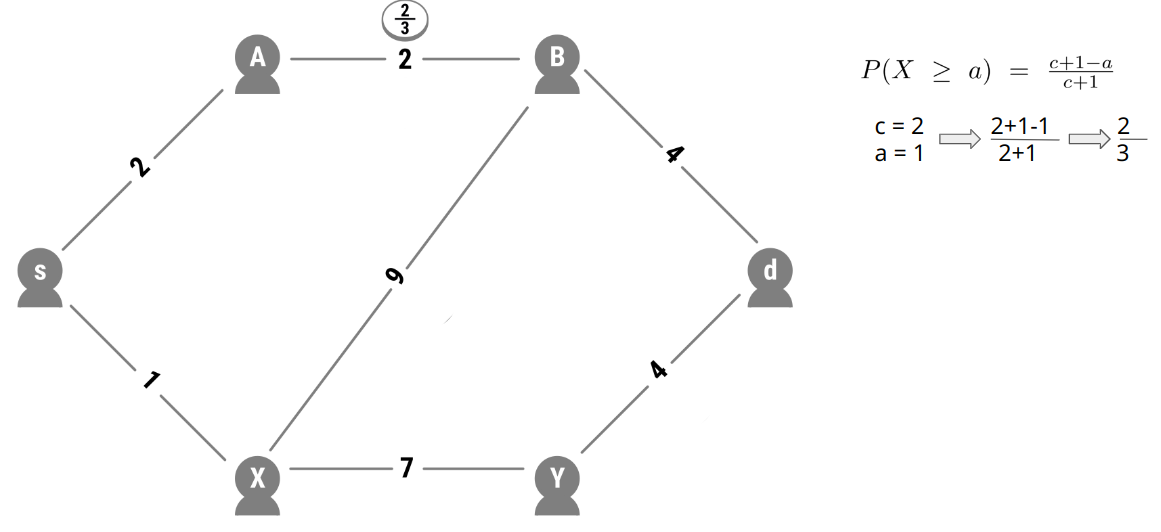
\includegraphics[width=0.6\columnwidth]{imgs/mincost_rene1.png}
  \end{center}
  \caption{Lightning Network Payment from A to B using channel success probability score.} 
  \label{fig:channel_success_prob_score}
\end{figure}


However, the paper shows also that with gossip data is difficult to simulate 
a real environment, and this means that the model described does not take into 
count the how fast an capacity $c(u, v)$ arrive to zero, or if this is a 
common case.

\subsection{Jamming Attach on Lightning}

The uncertain channel balances problem described in the previous section 
is not the only reason why payments on the lightning network are unreliable.
Another well-known problem on the Lightning Network is \emph{jamming attack},
it is a cheap denial-of-service (DoS) attack, where the goal of this DoS attack 
is to prevent payments, either routed through the victim or paying the victim. 
The effectiveness of jamming thus could be characterized by the reduction of 
payment success rate, applied to the victim or the entire Lightning Network.

The paper \cite{cryptoeprint:2022/1454} describe an solution to this problem 
based on a \emph{reputation system} and \emph{up-front fee} that allows to make
the Jamming attack is costly due to the up-front fee and difficult to do during the time 
due to the reputation system.
In addition, the paper defines different kinds of Jamming attacks, divided in :

\begin{itemize}
    \item {\bf Slow Jamming}: The attacker makes a payment with a very long timeout, 
        in this way all channel along the route has the balance locked;
    \item {\bf Fast Jamming}: The attacker tries to mimic the honest payment, by sending
        a failed payment; Currently, in the Lightning Network there is a similar operation
        that it is used to steal information from a channel called probing.
\end{itemize}

To mitigate slow and fast jamming the paper \cite{cryptoeprint:2022/1454}
propose a combination of two strategies, combined in the following way:

\begin{itemize}
    \item {\bf Up-front fee} paid to the downstream peer addresses quick jamming 
        by imposing a small cost on every payment;
    \item {\bf Local reputation} based on past behavior addresses slow jamming by 
        punishing peers who forward payments that take too long to resolve.
\end{itemize}

The solution proposed regarding the unconditional fee is relatively simple to implement 
because required a node to pay for an attempt also if this fails (if succeeded the up-front fee can 
be returned), and the choice of the path is driven by the local reputation that 
score the channel based on the following information:

\begin{itemize}
    \item  $\gamma$ (seconds): the maximal resolution time to consider a payment honest;
    \item  $\gamma$  (seconds), T (seconds), A (satoshis per second): reputation update 
    parameters;
    \item  K (integer), L(satoshis): the high-risk quota of slots and liquidity.
\end{itemize}


Calculating the Reputation Scores works by considering two possible values
for reputation scores:  \emph{high}  and  \emph{low}. Initially, all peers 
receive a low score. A payment is deemed  honest  if it resolves within  
$\gamma$  seconds, otherwise, it is considered a jamming attack. 
A peer’s behavior is defined as  good  if it only offers honest payments 
for forwarding. Moreover, those payments must pay at least A satoshis 
per second in fees to the routing node. The reputation of a peer grows if 
demonstrates good behavior for a long enough period.
